Para definir la metodología del presente plan de investigación se tomará como
referencia el libro \textit{Researching Information Systems and Computing}\cite{Oates2006}.
En él, Oates define seis aspectos fundamentales de la investigación, empleando
el mnemotécnico de las `6P'\footnote{Afortunadamente, el mnemotécnico se conserva con la traducción}:

Propósitos - o razones originales; productos - o entregables; proceso - actividades
realizadas durante la duración del proyecto; participantes - directos e indirectos;
paradigma - forma de interpretar la realidad; y la presentación - difusión y
comunicación del proyecto.

A continuación se concretan los diferentes aspectos mencionados.

\section{Propósitos}
\label{subsec:proposito}
Un proyecto de investigación necesita de un propósito claro para poder
definir las condiciones de finalización y éxito - total o parcial - del proyecto.

Es importante ser claro y sincero con el propósito último de este proyecto:
\emph{obtener el grado de doctor}. Aunque pueda parecer obvio dado el
contexto, es útil definir explícitamente una jerarquía de propósitos
``de arriba hacia abajo'' para limitar progresivamente el contexto del plan.

Una vez definido este propósito original, queda claro que, necesariamente,
el proyecto debe \emph{ampliar el cuerpo de conocimiento} del área en la que
se desarrolla. Si no se hubiera fijado la razón original, no habría ninguna
razón para no enfocar el plan desde un punto de vista puramente técnico o de
integración, por ejemplo.

Por otro lado, también se busca \emph{resolver un problema} real, que es
el análisis interactivo de gran cantidad de datos. El problema en concreto
se desarrolla con más detalle en la sección TODO NO FORWARD REFERENCES.

La intersección de estos propósitos generales es lo que motiva el presente plan,
que arranca con el análisis sistemático de la literatura\cite{Alvarez2019},
NO FORWARD REFERENCE, REMOVE THIS PARAGRAPH.

La hipótesis resultante se encuentra INTRODUCTION I GUESS??

\section{Paradigma}
\label{subsec:paradigma}
Aunque en el orden seguido por Oates el ``Paradigma'' es el quinto elemento,
se adelanta aquí a la segunda posición, ya que el marco filosófico 
determinará en gran medida el resto de aspectos, al delimitar
la forma de percibir la realidad, las reglas y los supuestos sobre los que
se sustentará la investigación\cite{Oates2006}. El paradigma define la naturaleza
del mundo, la relación del investigador con él, y cómo alcanzar el conocimiento.
Por definición, es un conjunto de ``creencias'' que no son posible demostrar
o discutir de forma racional\cite{Guba1994}.

Los diferentes paradigmas pueden definirse en función de las ``respuestas''
que dan a tres preguntas básicas\cite{Guba1990,Guba1994}: \emph{ontológica}
- naturaleza de la realidad; \emph{epistemológica} - relación entre el sujeto
y el conocimiento; y metodológica - vías de adquisición del conocimiento.

Diferentes autores pueden proponer diferentes clasificaciones, más o menos detalladas,
de los diferentes paradigmas. Por ejemplo, Guba\cite{Guba1990} propone cuatro -
positivismo, post-positivismo, teoría crítica y constructivismo -, mientras
que Chua\cite{Chua1986}, al igual que Oates\cite{Oates2006} describe tres ramas principales -
positivismo\footnote{``Mainstream'' en el original}, interpretativo y teoría crítica.
Shull \etal\cite{Shull2008} define igualmente estos tres paradigmas, más uno
adicional: el \emph{pragmatismo}.

El \emph{positivismo} considera que la realidad es objetiva, y el investigador
un observador imparcial. Por lo contrario, el paradigma \emph{interpretativo}
niega la existencia de una única ``verdad'', considerándola fruto del contexto
social del momento y del investigador.

Más activista es la \emph{teoría crítica}, donde el enfoque se pone en la
estructura social y las relaciones de poder. En definitiva, en el contexto
social.

Por último, el \emph{pragmatismo} (o realismo/relativismo\cite{Haack1977,Hookway2008,Pratt2016})
valora el conocimiento en función de la utilidad que se pueda obtener de él,
considerándolo en cualquier caso aproximado e incompleto\cite{Shull2008}.

\medskip

Considerando que en el presente plan de investigación es de una naturaleza
aplicada, se seguirá el paradigma del \textbf{Pragmatismo}.

\FloatBarrier

\section{Productos}
\label{subsec:productos}
Oates define cinco posibles tipos de contribuciones al conocimiento como productos, basándose
en una clasificación existente hecha por Davis \& Parker\cite{Oates2006,Davis1997}:
evidencia, metodología, análisis, teorías, y artefacto informático.

Como producto principal de esta investigación se espera obtener un nuevo
\emph{artefacto informático}, entendiendo como tal no solamente un elemento
software, sino también una nueva o perfeccionada \emph{técnica} que mejore
la exploración interactiva de datos como se ha descrito anteriormente.

Como productos secundarios también se pueden distinguir la revisión inicial de
la literatura\cite{Alvarez2019}, y los artículos académicos y presentaciones
que resulten de la investigación.

Por supuesto, la tesis final se considera también un producto.

\newpage

\section{Proceso}
\begin{figure}
  \centering
  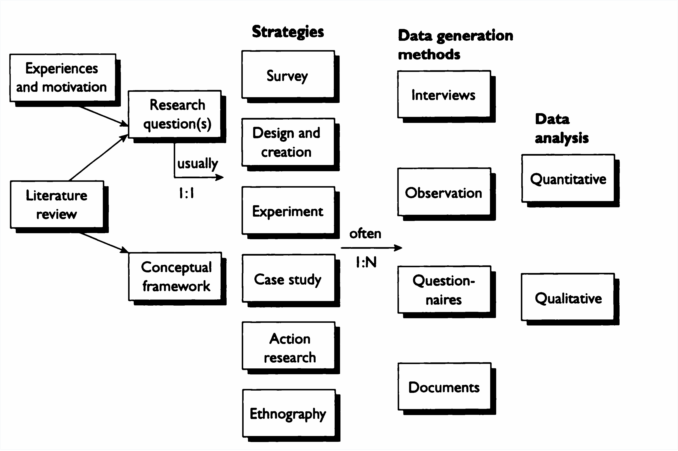
\includegraphics[width=\linewidth]{images/2_methodology/modelo_proceso.png}
  \caption{Modelo del proceso de investigación, extraído de \cite{Oates2006}}
  \label{fig:proceso}
\end{figure}

El modelo del proceso de investigación definido por Oates se resume en la
figura \ref{fig:proceso}.

La sección ?? contiene la motivación del proyecto;
la sección ?? incluye una revisión sistemática de la literatura;
y la hipótesis está definida en la subsección ??.

Necesitamos, pues, definir las estrategias, métodos, y el tipo de análisis de
datos que se seguirán. Estos puntos, junto con las secciones previamente mencionadas,
definirán el marco conceptual del proyecto.

\subsection{Estrategias}
\paragraph{Diseño y creación} Es la estrategia más adecuada para el presente
proyecto, ya que se busca obtener un algoritmo - y una implementación inicial -
que demuestre si la hipótesis planteada es viable.

Dentro de estar estrategia es necesario definir, además, la metodología de
desarrollo a seguir. Se optará por el método \textit{Engineering Design}:
    
\begin{quote}\textit{
  Engineering design is the systematic, intelligent generation and evaluation of
  specifications for artifacts whose form and function achieve stated objectives
  and satisfy specified constraints.}\cite{Dym2012}
\end{quote}

En la figura \ref{fig:engineering_design} se muestran las diferentes etapas
de este método de desarrollo.
 
\begin{figure}
  \centering
  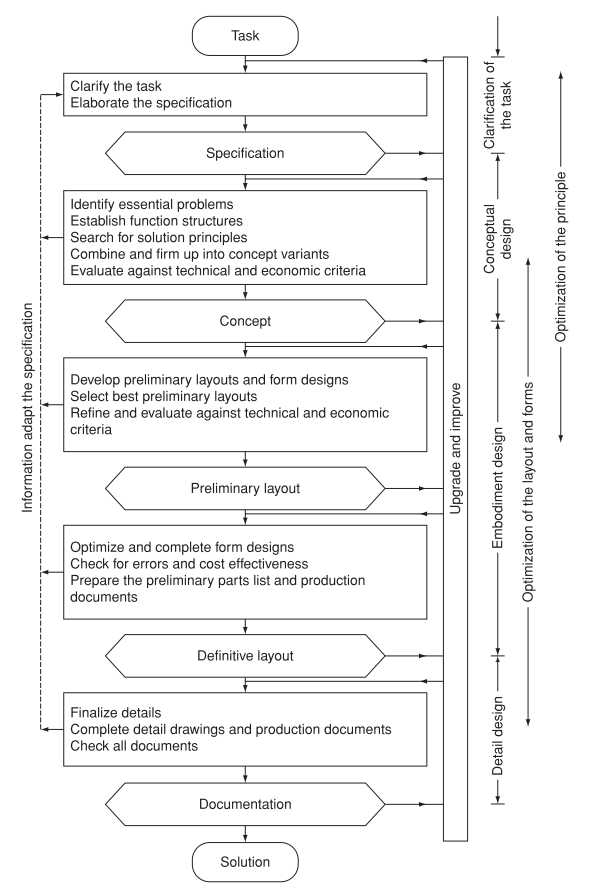
\includegraphics[width=\linewidth]{images/2_methodology/design_process.png}
  \caption{Proceso de diseño\cite{Dym2012,Pahl1984}}
  \label{fig:engineering_design}
\end{figure}
    
\paragraph{Experimentos} De forma complementaria, se necesitará comparar
el rendimiento de distintas implementaciones, y de diferentes niveles de
optimización. En definitiva, se deberán realizar \emph{experimentos controlados},
garantizando la validez interna del estudio.

\subsubsection{Métodos de generación de datos}
Para mejor definir los casos de uso, y para buscar conjuntos de datos
útiles para realizar las comparativas, se utilizarán \textbf{documentos}
existentes, entendiendo como documento desde artículos científicos (casos de uso)
hasta bases de datos.

Por otro lado, por la parte experimental se realizarán \textbf{observaciones}
(medidas) de cómo diferentes algoritmos y parámetros influyen en el rendimiento
final de diferentes sistemas e implementaciones.

\subsubsection{Análisis de datos}
Los datos se analizarán fundamentalmente de forma \emph{cuantitativa}, dado
que los distintos algoritmos e implementaciones se compararán en base a
medidas numéricas como puede ser tiempo de ejecución, bytes leídos, etc.


\section{Participantes}
Los únicos participantes directos el estudiante de doctorado
y los directores de tesis. Indirectos serán los editores y revisores de
potenciales revistas científicas y técnicas.

No se planea, por el momento, involucrar a terceras personas como sujetos
de investigación, aunque tampoco se descarta la posibilidad de alguna encuesta.
En cualquier caso, si la hubiera, se tendrán en cuenta los derechos básicos\cite{Oates2006}:
a no participar, a retirarse, a ser adecuadamente informados, al anonimato
y a la confidencialidad.

Si hubiera algún tipo de estudio que involucre, como sujetos, a otras personas,
se desarrollará con más detalle cómo se garantizarán estos cinco derechos.

\section{Presentación}
El total del trabajo realizado se compilará en una tesis final. No obstante,
durante el desarrollo se espera presentar los resultados obtenidos en
conferencias, publicaciones académicas, demostraciones técnicas, etc.

Es importante identificar publicaciones y foros de reconocido prestigio dentro
del área de investigación del presente proyecto.

\todo{Move to 2. Methodology the Literature Mapping from Chapter 3}

Research question introduction, literature review chap.3 (link with methodology here).
Data generation, observations (experiments), Data Analysis quantitative and qualitative (SOM),
link with chapter about discussion/results?

Task -> Specification -> Concept -> Preliminary chap 4 (bridge, plus preliminary excuse for dead ends)
Definitive layout 5 and 6 (presq and som).

\section{Systematic Mapping}
\todo{Move part of 3.2 here}

\section{\textsc{OpenScience}}
\todo{https://openscience.eu/}

\begin{quote}
    The FAIR principles (Findable, Accessible, Interoperable and Reusable) will become the basis for research work. Several measures and methods need to be implemented in research and innovation projects to foster dissemination, communication and exploitation of research outputs. 
\end{quote}
